\documentclass[12pt]{extarticle}
%% usepackage taken from https://tex.stackexchange.com/a/327136/135365
%%   thanks https://tex.stackexchange.com/users/4427/egreg
\usepackage[
  top=2cm,
  bottom=2cm,
  left=3cm,
  right=2cm,
  headheight=27pt, % as per the warning by fancyhdr
  %includehead,includefoot,
  heightrounded, % to avoid spurious underfull messages
]{geometry} 
\usepackage{lipsum}
\usepackage{setspace}
\usepackage{graphicx}
\usepackage{url}
\usepackage{xspace}
\usepackage{color}
\usepackage{amsthm}

\usepackage{pgfplots}
    \usetikzlibrary{calc}
    \pgfplotsset{compat=1.11}

\input{definitions}
\input{theorems}


\title{Day of Immersion: Programming in the Cloud: Roots of Polynomials}
\author{Dr. Jim Newton}
\begin{document}
\maketitle
\sloppy
%\thispagestyle{empty}
\section{Introduction}
\label{sec.intro}

In this atelier you will develop a software program in the cloud.  After
initially setting up your programming environment using GitHub Code Spaces, you
will develop a \code{hello-world} program in the
Python programming language.  You will then proceed to write functions
to compute roots of polynomials step by step starting with polynomials
of degree~1, and ending with polynomials of degree~5.

There is not enough time in this short atelier to complete the entire
development.  However, because the development is entirely in the
cloud, you may finish the development as quickly or as leisurely as
you like in the coming days, weeks, months.

\subsection{Overview}

You will finish the development of a program which will compute the
roots of polynomials of degree~1 through~5.
\begin{align*}
  a x + b\\
  a x^2 + b x + c\\
  a x^3 + b x^2 + c x + d\\
  a x^4 + b x^3 + c x^2 + d x + e\\
  a x^5 + b x^4 + c x^3 + d x^2 + e x + f
\end{align*}

The suite of Python functions you will implement (finish the
implementation of) are designed to review your mastery of
\begin{itemize}
\item Polynomials
\item Factorization
\item Quadratic formula
\item Finding Extrema using the Derivative
\item and more
\end{itemize}

\subsection{Flow of Today's Atelier}
You should advance as far as possible in this flow today.  You don't have
enough time to complete all the sections today.  However, if you find the
atelier interesting and challenging, then you may finish it at home at
your leisure.

\begin{enumerate}  

\item \textbf{Set up your cloud environment:}

  In \S\ref{sec.github} (page~\pageref{sec.github}) you will setup your cloud environment. You
  will then examine and modify a simply \code{hello world} program.

\item \textbf{Hello World:}

  Starting in \S\ref{sec.hello.world} (page~\pageref{sec.hello.world}), write the
  \emph{Hello World} program to help you learn how to use the GitHub
  Code Space programming environment.  Complete file \code{hello.py}.

In the remaining sections, starting with \S\ref{sec.line} (page~\pageref{sec.line}), you
will develop Python code to compute the roots of polynomials.  


\item \textbf{Optional: Review of Algebra}

  \S\ref{sec.general} (page~\pageref{sec.general}) which explains the math
  connected to the program you will develop.


\item \textbf{Roots of a line:}

  In \S\ref{sec.line} (page~\pageref{sec.line}) you'll find the sole root of a 1st
  degree polynomial (called a line).  Complete file \code{line.py}.
  Use \S\ref{sec.line} (page~\pageref{sec.line}) to understand the theory.

\item \textbf{Roots of a quadratic:}

  You'll complete the file
  \code{quadratic.py}.  You'll find at most two roots of a 2nd degree
  polynomial (called a quadratic).  Use \S\ref{sec.quadratic} (page~\pageref{sec.quadratic}) to
  understand the theory.

\item \textbf{Roots of a cubic:}

  In \S\ref{sec.cubic} (page~\pageref{sec.cubic}), you'll find at most
  three roots of a 3rd degree polynomial (called a cubic).  Complete
  the code in \code{cubic.py}.

\item \textbf{Roots of quartic and quintic:}

  If there's time remaining in the
  atelier, \S\ref{sec.quartic} (page~\pageref{sec.quartic}) and \S\ref{sec.quintic} (page~\pageref{sec.quintic}) deal with
  4th and 5th order polynomials.  Even if there's not enough time to
  finish all the exercises in this atelier, you may continue the work
  on your own time, because your account of GitHub will remain in
  place as long as you do not delete it.
  
\end{enumerate}


Good Luck! And Happy Coding.


% LocalWords:  atelier Atelier GitHub quartic quintic
\pagebreak
\section{Programming in the Cloud with GitHub}
\label{sec.github}


\begin{figure}[h]
  \centering
  \includegraphics[width=0.5\textwidth]{GitHub-How-to-use-GitHub-Edureka-300x241.png}
%%  \url{https://www.edureka.co/blog/how-to-use-github/}
  \caption{GitHub is a cloud service that hosts code repositories which 
    you can access via a web browser.}
\end{figure}

\subsection{Objectives}
The assignment in this section is:
\begin{enumerate}
\item Create a GitHub account
\item Open the \code{src/hello.py} with GitHub Code-Spaces.
\item Run the \emph{tests}  in \code{tests/test\_hello.py}using Code-Spaces
\end{enumerate}



\clearpage
\subsection{Create a GitHub Account}
\label{sec.account.create}
\begin{itemize}
\item \textbf{If you already have a GitHub account}: skip this section
(Section~\ref{sec.account.create}) and go directly to
Section~\ref{sec.github.login} (page \pageref{sec.github.login}).


\item \textbf{If you do not yet have a GitHub account}: you must create one.
Create a GitHub account using an abstract user name.  Don't use your
real name.  Instead use an artificial name use as your name from
Instagram or other social media.  You may also make up a completely
new name as long as no other person has already used that name on
GitHub.  \url{https://github.com/join}.  To complete the process of
creating a GitHub account you may need to authenticate using your
mobile phone.
\end{itemize}


\noindent\includegraphics[width=0.55\textwidth]{github-join.png}


\subsection{Log In to GitHub}
\label{sec.github.login}

If you are not already logged into GitHub, you should login at \url{http://github.com}.

\noindent
\includegraphics[width=0.8\textwidth]{github-signin.png}


\clearpage
\subsection{Open the Repository}
\label{sec.open.repo}
  


Open \url{https://github.com/jimka2001/immersion} with your web browser.  This makes the project visible to you.

\noindent\includegraphics[width=0.7\textwidth]{github-immersion.png}


\subsection{Fork yourself a copy}

Fork the repository.  This gives you a private copy.  You will make changes
necessary changes in the code using this private copy.

\noindent \includegraphics[width=0.6\textwidth]{github-fork-repo.png}



\subsection{Open a Python File in Code-Spaces}
  
\begin{enumerate}
\item Navigate to \code{src/hello.py} in the GitHub file browser, to see something like this.

\noindent\includegraphics[width=0.9\textwidth]{find-hello.png}



\item Click \code{hello.py} to open the file in an editor pane.  You
  should see something like what is shown here:

\noindent\includegraphics[width=0.9\textwidth]{hello-function.png}


\item Open the file by clicking \code{github.dev} not \code{Edit in place}.

\noindent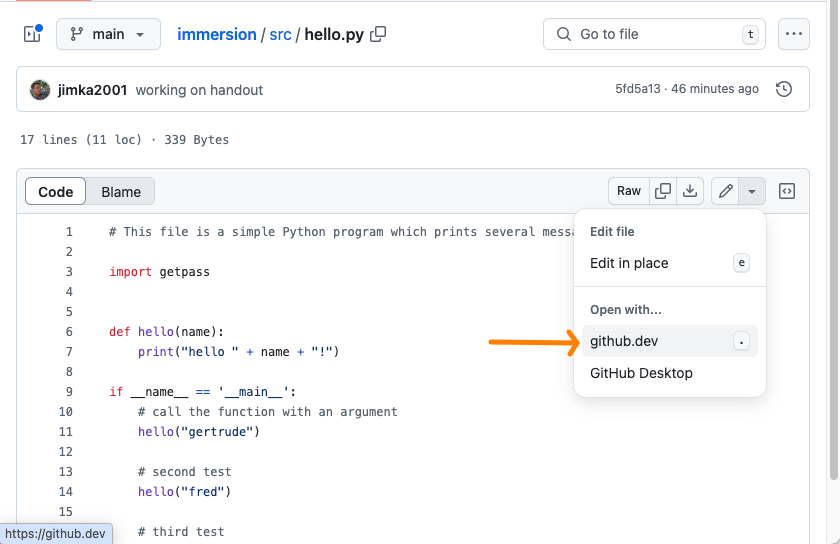
\includegraphics[width=0.9\textwidth]{github-dev.png}


\item You may need to wait while setting up. If this setup seems to
  never finish, it may mean you need to use Chrome as your web
  browser.

\noindent\includegraphics[width=0.4\textwidth]{github-dev-setup.png}


\item GitHub may ask for permission to see your repository.  Click on \textbf{Allow}.
  
\noindent\includegraphics[width=0.7\textwidth]{github-ask-permission.png}
  

\item GitHub may ask for your GitHub ID.  Normally you just select the default one.
  
\noindent\includegraphics[width=0.5\textwidth]{github-ask-user-name.png}

\item Finally, the GitHub development environment should be opened.
  
\noindent\includegraphics[width=0.6\textwidth]{github-dev-opened.png}



\end{enumerate}

\subsection{Set up the Editor}
  
\begin{enumerate}

\item Now you can edit your code but you cannot run nor test it.

\item Find the icon \includegraphics[width=2cm]{run-debug.png} on the
  left hand side of the browser window.  Press that icon to see the
  following message.

\noindent\includegraphics[width=0.6\textwidth]{continue.png}

\item Press continue, and you should see a prompt such as the
  following to create a code space.

\noindent\includegraphics[width=0.9\textwidth]{create-code-space.png}

\item Select \includegraphics[width=8cm]{select-create.png}.

\item You may be asked how many cores do you want.

\noindent\includegraphics[width=0.9\textwidth]{select-cores.png}

\item You should select the minimum: \includegraphics[width=7cm]{two-cores.png}.

\item You'll probably now need to reopen the \code{src/hello.py} file.

\noindent\includegraphics[width=0.9\textwidth]{re-open-python-file.png}

\item You may be asked to install the Python extension.  Press \textbf{Install}.

\noindent\includegraphics[width=0.8\textwidth]{install-python-extension.png}

  

\item Wait until it finishes installing.  When it finishes installing,
  you should see something like this:

\noindent\includegraphics[width=0.9\textwidth]{python-extension.png}

\item Reopen the explorer: \includegraphics[width=7cm]{explorer2.png},
  and select the \code{src/hello.py} file.

\noindent\includegraphics[width=0.4\textwidth]{explorer.png}
\end{enumerate}

\clearpage


% LocalWords:  GitHub atelier IDE CodeSpaces github
\pagebreak
\section{Test the IDE with Hello World}
\label{sec.hello.world}

The first program we usually write in any programming language is
called \code{hello-world}.  It is a very simple program.  However
getting it to run means you have to understand how to use the
programming environment.

\subsection{Examine the Code}
\label{sec.examine.the.code}
Take a look at the Python code in the file \code{src/hello.py}.  In
particular there are two sections in the code,
\begin{enumerate}
\item A declaration of the function named \code{hello}, shown in
  Listing~\ref{list.hello}
\item Two conditional calls to the function \code{hello}, each time
  with a different argument, shown in Listing~\ref{list.calls}.
\end{enumerate}

\begin{listing}{Declaration of Function \code{hello}}{hello}
\begin{minipage}[c]{0.95\textwidth}\begin{lstlisting}
def hello(name):
    print("hello " + name + "!")
\end{lstlisting}\end{minipage}\end{listing}

\begin{listing}{Calls to Function \code{hello}}{calls}
\begin{minipage}[c]{0.95\textwidth}\begin{lstlisting}
if __name__ == '__main__':
    # call the function with an argument
    hello("gertrude")
    
    # second test
    hello("fred")
\end{lstlisting}\end{minipage}\end{listing}


\subsection{Make a Sample Run}

Find the icon \includegraphics[height=1.0cm]{run-triangle.png} in the
top-right of the editor window.  Click the triangle, to see a sample
run/execution of the code.

\noindent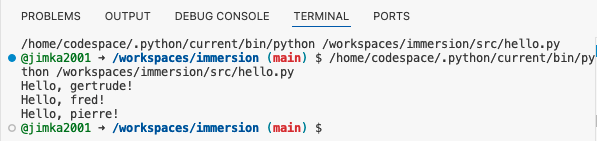
\includegraphics[width=\textwidth]{hello-terminal-output.png}


\subsection{Running Predefined Tests}
\label{sec.run.tests}

Open the file \code{tests/test\_hello.py} in a GitHub Code-Space.

\noindent\includegraphics[width=0.4\textwidth]{test-hello-explorer.png}

To run the tests, press the
\includegraphics[width=1cm]{run-triangle.png} which you should find in
the upper-right corner of the editor window.

\noindent\includegraphics[width=0.8\textwidth]{hello-test.png}


The text window at the bottom of the editor should show the results of
how many tests ran and whether there are any failures.

\noindent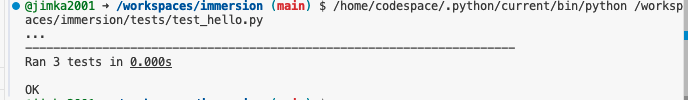
\includegraphics[width=0.9\textwidth]{github-test-result.png}



\subsection{Challenges for the Student}

Understanding errors and debugging is difficult, but it is part of
programming.

Experiment with the simple pieces of code in the above sections.
Insert spaces and press the run button.  Look at the error messages
produced. Remove some quotation marks or parentheses (leaving
unbalanced quotations marks or parentheses)---again look at what error
messages you see when you try to run invalid code.


\begin{enumerate}
\item Remove and add some spaces at the beginning of a line.
\item Change the indentation.
\item Unbalance the parentheses.
\item Unbalance the quotation marks.
\item Put extra spaces inside the quotation marks.
\item Change the name of the \code{hello} function at definition site
  or call site.
\item Figure out how to undo your changes in the editor to make the
  code work again.
\item Run the tests \code{test/test\_hello.py} as explained in
  Section~\ref{sec.run.tests}.
\end{enumerate}

\clearpage

% LocalWords:  GitHub png github
\pagebreak\mbox{}\pagebreak
%\setcounter{page}{0}
%\thispagestyle{empty}
\section{Review of Polynomials (Optional)}
\label{sec.general}

Your goal in the next several sections is to find \emph{root} of
\emph{polynomials}.  This section (\S\ref{sec.general}) explains
the how and why the algorithm works.  The algorithm is summarized
in \S\ref{sec.algorithm} (page~\pageref{sec.algorithm})

If you want to start coding quickly, you skip directly to
\S\ref{sec.line} (page~\pageref{sec.line}).  If you are also
interested in the theory, you can quickly read over
\S\ref{sec.general}.


\subsection{What is a Polynomial?}

\begin{definition}{polynomial of degree n}{}
  A \emph{polynomial} of \emph{degree n} is a function of a single
  variable, usually $x$, of the form.
  \[P(x) = \alpha_n x^n + \alpha_{n-1} x^{n-1} + \cdots + \alpha_2 x^2 + \alpha_1 x + \alpha_0 \]

  where $\alpha_n, \alpha_{n-1}, \ldots, \alpha_0$ are called
  coefficients and may be integers, rational numbers, or real numbers.
\end{definition}

$P(x) = 2 x^4 + 5 x^3 + x^2 - x + 1$ is 4th degree polynomial.


Any of the coefficients after the leading one may be 0.  Terms with a coefficient of zero
are usually omitted.  $P(x) = 5 x^3 + x - 1$ is 3th degree polynomial
where the coefficient of the $x^2$ term is 0.


\subsection{Fundamental Theorem of Algebra}

\begin{definition}{root}{}
  If $P(x)$ is a polynomial, and $r$ is a number for which $P(r)=0$,
  then $r$ is called a \emph{root} of the polynomial.
\end{definition}

The polynomial $P(x) = x^3 - x$ as three roots, 1, -1, and 0.  We know
this because
\begin{align*}
  P(1) &= (1)^3 - 1 
  = 1 - 1 
  = 0\\[3pt]
  P(-1) &= (-1)^3 - (-1) 
  = -1 + 1 
  = 0\\[3pt]
  P(0) &= (0)^3 - 0
  = 0 - 0 
  = 0  
\end{align*}

The fact that $P(x) = x^3 - x$ has \emph{at least} three roots is easy
to verify simply by evaluating the function $P(x)$ at 1, -1, and 0.
Theorem~\ref{th.n.roots} claims something stricter; it claims that $P(x)$
has at most three roots.  But before getting to Theorem~\ref{th.n.roots}, we take a look at Theorem~\ref{th.ftoa}.


\begin{theorem}{Fundamental Theorem of Algebra}{ftoa}
  Every non-constant polynomial of degree~1 or higher has a root.
\end{theorem}

The Fundamental Theorem of Algebra claims that every polynomial has a root.
However, sometimes the root is complex.  For example the polynomial,
$P(x) = x^2 + 1$, has two (and only two) complex roots, where $i=\sqrt{-1}$.

\begin{align*}
  P(i) &= i^2 + 1 
  = -1 - 1 
  = 0\\[3pt]
  P(-i) &= (-i)^2 + 1 
  = (-1)^2(i)^2 + 1 = (1)(-1) + 1
  = 0
\end{align*}


From this point forward, in this atelier, we only
attempt to determine the real roots, ignoring the complex roots.  For
this reason, we will not be able to find all the roots of some
polynomials.

\begin{theorem}{Roots with Multiplicity}{n.roots}
  A polynomial of degree $n\ge 1$ has $n$ roots, some of which may be
  equal.
\end{theorem}
\begin{proof}

  [By Induction]
  
  \begin{itemize}
    
  \item \textbf{Base case:} If $n=1$, then Theorem~\ref{th.ftoa}
    guarantees it has a root; call it $r_1$.  Thus it is of the form
    $P(x)=\alpha (x-r_1)$.
  \item \textbf{Inductive case:} Suppose $n>1$.  Suppose every
    polynomial, $Q(x)$ of degree $n$ has $n$-many roots,
    $r_1,\ldots,r_n$, and can thus be written as:
    \[Q(x) = \alpha_1 (x - r_1) (x - r_2) \cdots (x - r_n)\]
    Now consider a polynomial, $P(x)$, of
    degree~$n+1$.  Theorem~\ref{th.ftoa} guarantees $P(x)$ has a root;
    call it $r_{n+1}$, thus $(x-r_{n+1})$ is a factor of $P(x)$ so there
    exists a polynomial, $Q(x)$, of degree~$n$ such that
    $P(x) =  Q(x) (x-r_{n_1})$.
    But by inductive hypothesis, $Q(x)$ can be written
    as \[Q(x) = \alpha_1 (x - r_1) (x - r_2) \cdots (x - r_n)\]
    So, \[P(x) = \alpha_1 (x - r_1) (x - r_2) \cdots (x - r_n) (x-r_{n+1})\]

    Thus $P(x)$ has $n+1$ roots.
  \end{itemize}
\end{proof}

\subsection{Algorithm for Finding Roots}
\label{sec.algorithm}

The proof of Theorem~\ref{th.n.roots} gives us the algorithm which we will use to find
roots in this atelier.  Given a degree~$n$ polynomial (for $2<n\leq5$),
\begin{enumerate}
\item If we successfully find a root, $r_n$ of the $n$-degree polynomial
\item Then we will factor  $(x-r_n)$ out of the polynomial,
\item Giving us new polynomial but with degree~$n-1$,
\item Which we can solve by the same approach.  
\item This process continues until we reach degree~$n=2$ which we
  solve using the quadratic formula.

\end{enumerate}


% LocalWords:  atelier
\pagebreak
\input{sec-line}\pagebreak
\section{Quadratic: degree=2}
\label{sec.quadratic}

\subsection{Objectives}
The assignment in this section is:
\begin{enumerate}
\item Complete the file \code{src/quadratic.py} by writing a Python
  function which computes and returns the x-intercepts of a parabola whose
  equation is \[y=a x^2 + b x + c\,.\]
\item    You'll need to replace all occurrences of \code{raise NotImplementedError()}
  with correct python code which passes the tests.

\item Test the function in GitHub Code-Spaces by running the file\\
  \code{test/test\_quadratic.py}.
\end{enumerate}

\subsection{Overview}

\begin{figure}
\centering
\input{pfg-parabola}
\caption{Parabolas}
\label{fig.parabola}
\end{figure}

A quadratic polynomial is of the form $P(x)=a x^2 + b x + c$.  If
$a=0$, then $P(x)$ is actually a first degree polynomial which can be
solved using the techniques described in \S\ref{sec.line};
otherwise we need a more elaborate technique which is explained here in
\S\ref{sec.quadratic}

We have the plots of three quadratic polynomials, $P_1(x)$, $P_2(x)$,
and $P_3(x)$, shown in Figure~\ref{fig.parabola}.  Each plot takes the
geometric form of a parabola.  As can be seen in the figure, the
parabola might intersect the x-axis twice (\eg, $P_1(x)$), once (\eg,
$P_2(x)$, or not at all (\eg, $P_3(x)$).

\begin{align*}
  P_1(x) &= 2x^2 - 2 x - 1\\
  P_2(x) &= x^2 -x + \frac{1}{4}\\
  P_3(x) &=  -2x^2 + 2x -2
\end{align*}


\subsection{The Math / The Theoretical}

To determine how many times a parabola touches the x-axis, we need to
find the roots of the corresponding quadratic (degree~2) polynomial of
the form $a x^2 + b x + c$.  The formula is called the \emph{quadratic
formula}:

\[x = \frac{-b\pm\sqrt{b^2 - 4a c}}{2a}\]

In particular,
we need to look at the expression under the square root, called the
discriminant: $b^2 - 4a c$.
\begin{itemize}
\item If the discriminant is positive, then the polynomial has two
  distinct real roots.
\item If the discriminant is zero, then the positive and negative
  square roots $\pm\sqrt{b^2 - 4a c}$ in the quadratic formula are
  both 0; thus the polynomial has 1 single root where the parabola
  touches the x-axes tangentially.
  
\item If the discriminant is negative, then there is a negative under
  the radical sign; thus the polynomial has no real roots.  The
  polynomial does have complex roots; however we will ignore complex
  roots for this atelier.
\end{itemize}

\subsection{The Programming / The Practical}

Steps for computing roots of a polynomial of degree~2.
\begin{enumerate}
\item Assume the coefficients of $P(x)$ are in the variables \code{a},
  \code{b}, and \code{c}.
\item If \code{a == 0}, then delegate to previous solution by calling
  the function \code{find\_x\_intercept} and returning its value.
  Note that \\ \code{find\_x\_intercept} takes two arguments, which it
  calls \code{a} and \code{b}, but these are not \code{a} and \code{b}
  of the quadratic.  In fact for \code{find\_x\_intercept}, \code{a}
  is the coefficients of $x$ and \code{b} is the bias term of $a x +
  b$.  However, for the quadratic, \code{a} is the coefficient of
  $x^2$, and \code{b} is the code of $x$ in $a x^2 + b x + c$.
\item Compute the discriminant, storing in the variable
  \code{discriminant}.
\item Test three conditions.
  \begin{enumerate}
  \item If the discriminant is positive, then return a list of the two
    roots.
  \item If the discriminant is zero (or very close to zero), then
    return a list (of length one) of the root.
  \item If the discriminant is negative ( $< -\varepsilon$), then
    return an empty list~\code{[]}.
  \end{enumerate}

\item Test your code by running the pre-defined tests in
  \\ \code{tests/test\_quadratic.py}.

\item Look at the proposed solution in \code{solutions/quadratic.py}.
  It is not necessary that your code match exactly.


\end{enumerate}


\begin{listing}{Function to compute roots of a quadratic polynomial.}{code.quadratic}
\begin{minipage}[c]{0.95\textwidth}\begin{lstlisting}
def find_quadratic_roots(a, b, c):
    epsilon = 0.001
    discriminant = b * b - 4 * a * c
    if a == 0:
        # CHALLENGE: student must complete the implementation.
        raise NotImplementedError()

    if abs(discriminant) < epsilon:
        # CHALLENGE: student must complete the implementation.
        raise NotImplementedError()

    elif discriminant > 0:
        # CHALLENGE: student must complete the implementation.
        raise NotImplementedError()

    else:
        # CHALLENGE: student must complete the implementation.
        raise NotImplementedError()

\end{lstlisting}\end{minipage}\end{listing}


% LocalWords:  NotImplementedError abs elif atelier GitHub Parabolas
\pagebreak
\section{Cubic: degree=3}
\label{sec.cubic}

\subsection{Objectives}
The assignment in this section is:
\begin{enumerate}
\item Complete the file \code{src/cubic.py} by writing a Python
  function which computes and returns the x-intercepts of a curve
  equation is \[y=a x^3 + b x^2 + c x + d\,.\]
\item You'll need to replace all occurrences of \code{raise NotImplementedError()}
  with correct python code which passes the tests.

\item Complete the file \code{src/search.py} by completing the function \\
  \code{search\_root\_right}
  which follows a similar pattern to that of \\
  \code{search\_root\_left} which you have all the code for.

\item Test the function in GitHub Code-Spaces by running the file\\
  \code{test/test\_cubic.py}.
\end{enumerate}

\subsection{Overview}

We wish to find the roots of the cubic polynomial given by $P(x) = a
x^3 + b x^2 + c x + d$.  We will do this by first finding
(approximating) a root, $r$, using a technique called \emph{binary
search}.  Knowing root $r$, we know that $(x-r)$ is a factor of $a x^3 + b x^2 + c x + d$.
Once $(x-r)$ is factored out of $a x^3 + b x^2 + c x + d$
what remains is a quadratic polynomial of the form $A x^2 + B x + C$.
We can find the roots of the quadratic using the technique
explained in Section~\ref{sec.quadratic}, thus obtaining the roots of
the cubic polynomial.


\subsection{The Math / The Theoretical}
\label{sec.cubic.math}
A polynomial of degree~3 has the form $P(x) = a x^3 + b x^2 + c x +d$.
If $a=0$ then $P(x)$ is really a quadratic polynomial (degree~2)
and can be solved using the techniques described in
Section~\ref{sec.quadratic}.  Every polynomial of degree~3 with real
coefficients (for which $a\neq 0$) has at least one real root because
\begin{enumerate}
\item Either $\lim\limits_{x\to-\infty}P(x) = -\infty$ and $\lim\limits_{x\to\infty}P(x) = \infty$,
  \item Or $\lim\limits_{x\to-\infty}P(x) = \infty$ and $\lim\limits_{x\to\infty}P(x) = -\infty$.
\end{enumerate}


We have a two cubic equations plotted in Figure~\ref{fig.cubic}.

\begin{figure}
  \centering
\input{pfg-cubic}
  %
  \caption{Cubics}
  \label{fig.cubic}
\end{figure}

\begin{align*}
  P(x) &= x^3 - 4 x^2 - 2 x - 10\\
  -P(x) &= -x^3 + 4 x^2 + 2 x + 10
\end{align*}

$P(x)$ exemplifies the \emph{standard} case where the leading coefficient is positive: $a>0$.
$-P(x)$ exemplifies the alternate case where the leading coefficient is negative: $a<0$.
However, we notice that $P(x)$ and $-P(x)$ have the exact same roots, because if $-P(x) = 0$,
then $P(x) = 0$.  Therefore, if $a<0$, we can simply find the roots of $-a x^3 -b x^2 - c x - d$;
\ie, we simply negate the coefficients and find the roots of the negated cubic polynomial.




Given a cubic polynomial and a root, $r$, we may factor the polynomial into
the product of a monomial $(x-r)$ and a quadratic polynomial.

If $P(x) = a x^3 + b x^2 + c x + d$ has a root at $x=r$, then $P(r)=0$.
Consequently, $(x-r)$ is a factor of $a x^3 + b x^2 + c x + d$, and
$P(x) = (x-r)(A x^2 + B x + C)$ for some $A, B, C$.  

\begin{align}
  P(x) &=  (a x^3 + b x^2 + c x + d)\nonumber\\
  &= (x-r) (A x^2 + B x + C)\label{eq.factor.ABC}
\end{align}

Once $A$, $B$,
and $C$ have been found, then the two remaining roots can be found by
applying the quadratic formula to $A x^2 + B x + C$.  So how can we
determine the values of $A$, $B$, and $C$ given the root $r$ and the
original coefficients $a$, $b$, $c$, and $d$?


We can verify that $A$, $B$, and $C$ are determined by the following equations.
\begin{align}
 A &= a\label{eq.6.A}\\
  B &= b + a r\nonumber\\
   &= b + A r\label{eq.6.B}\\
  C &= c + b r + a r^2\nonumber\\
  &= c + (b + a r) r\nonumber\\
  &= c + B r\label{eq.6.C}
\end{align}

The equations for $A$, $B$, and $C$ follow a regular and predictable
pattern which may not be immediately apparent.  However, the pattern
may become more clear when looking at the analogous derivation for
the quartic (Equations~\eqref{eq.7.A} through~\eqref{eq.7.D})
page~\pageref{eq.7.D}, and also for the quintic
(Equations~\eqref{eq.8.A} through~\eqref{eq.8.E}) page
~\pageref{eq.8.E}.

We may verify this factorization by substituting Equations~\eqref{eq.6.A}, \eqref{eq.6.B}, and~\eqref{eq.6.C}
into $(x-r) (A x^2 + B x + C)$, then working through some tedious algebraic manipulation.

\begin{align*}
  (x-r) (A x^2 + B x + C)
  &= (x-r) (a x^2 + (b + a r) x + (c + b r + a r^2))\\
  &= (x-r) (a x^2 + b x + a r x + c + b r + a r^2)\\
  &= x(a x^2 + b x + a r x + c + b r + a r^2) \\
  &\quad\quad - r (a x^2 + b x + a r x + c + b r + a r^2)\\
  &= a x^3 + b x^2 + a r x^2 + c x + b r x + a r^2 x\\
  &\quad\quad - a r x^2 - b r x - a r^2 x - c r - b r^2 - a r^3\\
  &= a x^3 + b x^2 + c x  \\
  &\quad\quad + \underbrace{a r x^2 + b r x + a r^2 x - ( a r x^2 + b r x + a r^2 x)}_{=0} \\
  &\quad\quad  - c r + b r^2 - a r^3\\
  &= a x^3 + b x^2 + c x + \underbrace{( d - d)}_{+0} - c r - b r^2 - a r^3\\
  &= \underbrace{a x^3 + b x^2 + c x +  d}_{=P(x)} - (\underbrace{d + c r + b r^2 + a r^3}_{=P(r)})\\
  &= P(x) - P(r)\\
  &= P(x) 
\end{align*}

Since $r$ is assumed to be a root of $P(x)$, then we know that $P(r)=0$.  Thus $P(x)-P(r)=P(x)$.

\subsection{The Programming / The Practical}

This challenge contains two parts:
\begin{itemize}
\item In \textbf{Find a root using Binary Search}, Section~\ref{sec.binary.search}, you will complete the file \code{src/search.py}.
\item In \textbf{Cubic Roots}, Section~\ref{sec.cubic.roots}, you will complete the file \code{src/cubic.py}.
\end{itemize}

\subsection{Find a root using Binary Search}
\label{sec.binary.search}

In this section you will complete the code in \code{src/search.py}.
This code will be reused in Section~\ref{sec.cubic.roots} and again in
Section~\ref{sec.quartic}.  The purpose of the code is to find one
root (any root) of a given polynomial.  The purposes of finding one
root is so we can factor $(x-r)$ out of the polynomial, thus reducing
a degree~3 polynomial to a degree~2, or in general reducing a degree~$n$ to a degree~$n-1$ polynomial.

\begin{figure}
  \centering
\input{pfg-cubic-binary1}
  %
  \caption{Expanding Binary Search} 
  \label{fig.cubic.binary}
\end{figure}

Consider the graph of the cubic polynomial shown in Figure~\ref{fig.cubic.binary}.  We'd like to
iteratively find a root; we will use the following steps.

\begin{enumerate}
\item If $P(0)=0$, then we know the root, $x=0$.
\item \label{step.2} If $P(0)< 0$, then find a value of $x_{upper}$ (to the right of 0, $x_{upper}>0$) such that either $P(x_{upper})>0$.
  Now take $x_{lower}=0$.
  Thus we
  will know there is a root in the interval $[x_{lower}, x_{upper}]$.
\item \label{step.3} If $P(0)> 0$, then find a value of $x_{lower}$ (to the left of 0, $x_{lower}<0$) such that either $P(x_{lower})<0$. 
  Now take $x_{upper}=0$.
 Thus we
  will know there is a root in the interval $[x_{lower}, x_{upper}]$.
\item \label{step.4} Since we know there is a root in the interval
  $[x_{lower}, x_{upper}]$, we can divide the interval into two
  intervals.  With the midpoint of the interval, \[x_{mid} =
  \frac{x_{upper} + x_{lower}}{2}\,,\] we consider two intervals:
  $[x_{lower}, x_{mid}]$ and $[x_{mid}, x_{upper}]$.  At least one of
  the following is true:
  \begin{enumerate}
  \item $x_{upper} - x_{right} < \varepsilon$, for some small epsilon (\eg, $\varepsilon = 0.00001$),
    then we know the root is $x_{mid} \pm \varepsilon$, which is good enough.
  \item $P(x_{mid}) = 0$, then we know the root $x= x_{mid}$.
  \item There is a root in the interval $[x_{lower}, x_{mid}]$, then
    we repeat step~\ref{step.4} on the interval $[x_{lower},
      x_{mid}]$.
  \item There is a root in the interval $[x_{mid}, x_{upper}]$, then
    we repeat step~\ref{step.4} on the interval $[x_{mid},
      x_{upper}]$.
  \end{enumerate}
\end{enumerate}


How does step~\ref{step.2} work?  Start with  $x_{upper}=1$, and query whether ${P(x_{upper}) < 0}$.
If so, then double $x_{upper}$ and try again, until ${P(x_{upper}) > 0}$.  As an example with the polynomial in Figure~\ref{fig.cubic.binary}, we would try ${P(1)< 0}$, ${P(2) < 0}$, ${P(4)<0}$, and finally ${P(8) > 0}$.

Similarly for step~\ref{step.3}?  Start with  $x_{upper}=-1$, and query whether ${P(x_{lower}) > 0}$.
If so, then double $x_{upper}$ and try again, until ${P(x_{upper}) < 0}$.


\subsection{Cubic Roots}
\label{sec.cubic.roots}

Steps for computing roots of a cubic polynomial.

\begin{enumerate}
\item Assume the coefficients of $P(x) = a x^3 + b x^2 + c x + d$ are
  \code{a},  \code{b},  \code{c},  and~\code{d}.
\item If \code{a==0}, then delegate to the previous solution by
  calling \\
  \code{find\_quadratic\_roots} and returning its return
  value.  Be careful, \code{find\_quadratic\_roots} accepts 3 input
  parameters.
\item If $P(x)$ is of the form of $-P(x)$ in Figure~\ref{fig.cubic},
  \ie, if $a<0$, then compute and return the roots of $-P(x)$.  To
  compute the roots of $-P(x)$ we simply return
  \code{find\_cubic\_roots(-a, -b, -c, -d)}.
\item Since $P(0) = d$, then we can easily evaluate the polynomial at $x=0$ to get its y-intercept.
  \begin{enumerate}
  \item If $d = 0$, then 0 is a root, $P(0) = 0$.
  \item If $d>0$ then there is a root on the negative x-axis.  Find it with a binary search.
  \item If $d<0$ then there is a root on the positive x-axis. Find it with a binary search.
  \end{enumerate}
\item See Section~\ref{sec.binary.search} to explain the binary search.
\item Once the root $r$ is found, this means $(x-r)$ factors out $P(x)$. \Ie,
  ${P(x) = (x-r)(A x^2 + B x + C)}$.  The formulas for $A$, $B$, and $C$ can be found
  in Equations~\eqref{eq.6.A}, \eqref{eq.6.B}, and~\eqref{eq.6.C}.
\item The roots of the cubic are \code{[r]} concatenated to the roots of the quadratic 
  $A x^2 + B x + C$, which you can compute using the techniques in Section~\ref{sec.quadratic}.


\item Test your code by running the pre-defined tests in \\
  \code{tests/test\_cubic.py}.

\item Look at the proposed solution in \code{solutions/cubic.py}.  It is not necessary that your code match exactly.



\end{enumerate}



% LocalWords:  NotImplementedError GitHub quintic quartic
\pagebreak
\section{Quartic: degree=4}
\label{sec.quartic}

\subsection{Objectives}
The assignment in this section is:
\begin{enumerate}
\item Complete the file \code{src/quartic.py} by writing a Python
  function which computes and returns the x-intercepts of a curve
  equation is \[y=a x^4 + b x^3 + c x^2 + d x + e\,.\]
\item You'll need to replace all occurrences of \code{raise
  NotImplementedError()} with correct python code which passes the
  tests.
\item Test the function in GitHub Code-Spaces by running the
  file\\ \code{test/test\_quartic.py}.
\end{enumerate}

\subsection{Overview}

We wish to find the roots of the quartic polynomial given by 
\[P(x) = ax^4 + b x^3 + c x^2 + d x + e\,.\]

We will do this by first finding (approximating) a root, $r$, using a
technique called \emph{binary search}.  We will determine which
regions to search by examining the derivative

\[\frac{d}{d x} P(x) = 4ax^3 + 3b x^2 + 2c x + d\,.\]

Knowing root $r$, we know that $(x-r)$ is a factor of
$a x^4 + b x^3 + c x^2 + d x + e$.  Once $(x-r)$ is factored out of $P(x)$ what remains
is a cubic polynomial of the form $A x^3 + B x^2 + C x + D$.  We can
find the roots of the cubic using the technique explained in
Section~\ref{sec.cubic}, thus obtaining the roots of the quartic
polynomial.


\subsection{The Math / The Theoretical}


A polynomial of degree~4 has the form $P(x) = a x^4 + b x^3 + c x^2 +
d x + e$. If $a=0$ then $P(x)$ is really a cubic polynomial (degree~3)
and can be solved using the techniques described in
Section~\ref{sec.cubic}.

If $a<0$ then similar to what we did for the cubic polynomial in
Section~\ref{sec.cubic.math}, we instead find the roots of
$-P(x) = -a x^4 - b x^3 - c x^2 - d x - e$.  $P(x)$ and $-P(x)$ are guaranteed to
have the same roots, but the code in Python will be easier if we know
that $a >= 0$.


Two polynomial equations (for $P(x)$ and $\frac{d}{d x} P(x)$) are
plotted in Figure~\ref{fig.quartic}.

\begin{figure}
\centering
\input{pfg-quartic}
\caption{Quartics}
\label{fig.quartic}
\end{figure}

\begin{align*}
  P(x) &= \frac{1}{8}  x^4 -2 x^3 + 7  x^2 + x + 6\\
  \frac{d}{d x} P(x) &= \frac{1}{2}  x^3 -6 x^2 + 14  x + 1
\end{align*}

Notice that at the extreme left and right, the plot of $P(x)$ opens
upward, and the graph changes direction 3 times.  The values of $x$ at
which $P(x)$ changes direction are called the \emph{inflection
points}.  The inflection points are local minima of $P(x)$, and can
be computed by finding the values for which $\frac{d}{d x} P(x) = 0$.
Since the derivative of a degree~4 polynomial is a degree~3 (cubic)
polynomial, we can find where $\frac{d}{d x} P(x) = 0$ by using the
techniques explained in Section~\ref{sec.cubic}.

Once we have determined the 3 inflection points $x_1$, $x_2$, and
$x_3$, we can simply test $P(x_1)$, $P(x_2)$, $P(x_3)$.  If one if
these values is 0, then we have found a root, $r$, and we can factor
$(x-r)$ out of $P(x)$ to obtain a cubic polynomial.  We can find the
roots of the cubic using the techniques explained in
Section~\ref{sec.cubic}.

If none of $P(x_1)$, $P(x_2)$, or $P(x_3)$ is zero, then we check
whether one of them is negative.  As shown in
Figure~\ref{fig.quartic}, whenever $P(x)<0$ then there is a root both
to the right and left of $x$.  If we can find that root, then as
before we can factor out $(x-r)$ to get a cubic polynomial, and then
find its roots--- thus obtaining the roots of the quartic.

Once we have determined a root, $r$ of $P(x)$, then we know (similar
to the cubic case in Section~\ref{sec.cubic.math}) that $P(x)$ factors
into $(x-r)(A x^3 + B x^2 + C x + D)$, where
\begin{align}
  A &= a\label{eq.7.A}\\
  B &= b + a r\nonumber\\
   &= b + A r\label{eq.7.B}\\
  C &= c + b r + a r^2\nonumber\\
  &= c + (b + a r)r\nonumber\\
  &= c + B r\label{eq.7.C}\\
  D &= d + c r + b r^2 + a r^3\nonumber\\
  &= d + ( c + b r + a r^2)r\nonumber\\
  &= d + C r\label{eq.7.D}
\end{align}

\subsection{The Programming / The Practical}

Steps for finding the roots of a quartic polynomial.

\begin{enumerate}
\item Assume the coefficients of $P(x) = a x^4 + b x^3 + c x^2 + d x + e$ are
  \code{a},  \code{b},  \code{c},  \code{d}, and~\code{e}.
\item If \code{a==0}, then delegate to the previous solution by
  calling \\
  \code{find\_cubic\_roots} and returning its return
  value.  Be careful, \\
  \code{find\_cubic\_roots} accepts 4 input
  parameters.
\item Since $P(0) = e$, then we can easily evaluate the polynomial at
  $x=0$ to get its y-intercept.
  \begin{enumerate}
  \item If $e = 0$, then 0 is a root, $P(0) = 0$.
  \item If $e<0$ then there is a root on the positive x-axis and a
    root on the negative x-axis.  Find it with a binary search.
  \end{enumerate}
\item Find the inflection points by finding the roots
  of \[\frac{d}{d x} P(x) = 4 a x^3 + 3 b x^2 + 2 c x + d\,.\]
  \begin{enumerate}
  \item If $P(x)$ is zero at one of these inflection points, then the
    inflection point is a root.
  \item If $P(x) < 0$ at an inflection point, then there is a root
    both to the right and the left; find with by calling either
    \code{search\_root\_right} or \code{search\_root\_left}.
  \end{enumerate}
\item Once a root has been found, factor \[P(x) = (x-r)(A x^3 + B x^2 +
  C x + D)\] by finding the coefficients, $A$, $B$, $C$, and $D$, using
  Equations~\eqref{eq.7.A} through~\eqref{eq.7.D}.
\item Find the roots of $A x^3 + B x^2 + C x + D$ using
  \code{find\_cubic\_roots}.
  \item Concatenate the list of all the roots together to obtain the
    roots of the quartic polynomial.

\item Test your code by running the pre-defined tests in
  \code{tests/test\_quartic.py}.

\item Look at the proposed solution in \code{solutions/quartic.py}.
  It is not necessary that your code match exactly.

\end{enumerate}

% LocalWords:  NotImplementedError quartic GitHub Quartics Quartic
\pagebreak
\section{Quintic: degree=5}
\label{sec.quintic}

This exercise is left as an exercise for the student.  However, the
following are some notes to help lead the student in the right
direction.

\begin{figure}
\centering
\input{pfg-quintic}
\caption{Quintic}
\label{fig.quintic}
\end{figure}

\begin{align*}
  P(x) &= x^5 - \frac{1}{2} x^4 + 5 x^3 + \frac{5}{2} x^2 + 4 x - 2
\end{align*}


A quintic polynomial has the form $P(x) = a x^5 + b x^4 + c x^3 + d x^2 + e x + f$.
If $a=0$ then $P(x)$ is really a quartic polynomial
(degree~4) and can be solved using the techniques described in
\S\ref{sec.quartic}.  Since a quintic polynomial has odd degree
(if $a\neq 0$), then, like the cubic (\S\ref{sec.cubic}), it is
guaranteed to have a real root.  This fact is guaranteed, because if
$a>0$ then $P(x)\to \infty$ for $x>>0$ and $P(x)\to -\infty$ for
$x<<0$.

Given this fact, we can find a root, $r$ using a binary search as we
did for the cubic.  Since $P(0) = f$, then we can consider two cases.
\begin{enumerate}
\item If $f>0$ then search for a root on the negative x-axis
\item If $f<0$ then search for a root on the positive x-axis
\end{enumerate}

Once the root $r$ is found, factor out $(x-r)$ from $P(x)$ to result
in a quartic, which we can solve using the technique in
\S\ref{sec.quartic}.
\begin{align*}
  P(x) &= a x^5 + b x^4 + c x^3 + d x^2 + e x + f\\
  &= (x - r) (Ax^4 + B x^3 + C x^2 + D x + E)
\end{align*}

Where

\begin{align}
  A &= a\label{eq.8.A}\\
  B &= b + a r\nonumber\\
   &= b + A r\label{eq.8.B}\\
  C &= c + b r + a r^2\nonumber\\
  &= c + (b + a r)r\nonumber\\
  &= c + B r\label{eq.8.C}\\
  D &= d + c r + b r^2 + a r^3\nonumber\\
  &= d + ( c + b r + a r^2)r\nonumber\\
  &= d + C r\label{eq.8.D}\\
  E &= e + d r + c r^2 + b r^3 + a r^4\nonumber\\
  &= e + ( d + c r + b r^2 + a r^3)r\nonumber\\
  &= e + D r\label{eq.8.E}
\end{align}


Having determined $A$, $B$, $C$, $D$, and $E$, the roots of
\[A x^4 + B x^3 + C x^2 + D x + E\] can be
found with a call to \code{find\_quartic\_roots}, which you
implemented in \S\ref{sec.quartic}.



% LocalWords:  Quintic quintic quartic




\end{document}

